% !TEX root = ./main.tex
% !TEX encoding = UTF-8 Unicode
% !TEX program = pdflatex
% !TeX spellcheck = it_IT

\graphicspath{{Immagini/},{Immagini/teoriaDelleCode/}}

\chapter{Teoria delle Code}

\section{Traccia}
\textit{A set of K=3 processes runnning on a computer can be modelled as a closed
network queueing.\\
Each process require CPU and I/O resources.\\
After executing on the CPU, for a time $ e^{5t} $ the process require the I/O with
probability $q=1/3$ before continue its execution.\\
The time for an I/O operation is $ e^{2t}$.\\
Analyze the queuing network using the MVA technique.\\
Implement the MVA algorithm in MATLAB, and find the solution of the previus excercise
varing the number K.\\
How varies the responce time of the I/O subsystem and the CPU subsystem, for
increasing the number of tasks? Plot the results.\\}

\begin{figure}[!htbp]
  \centering
  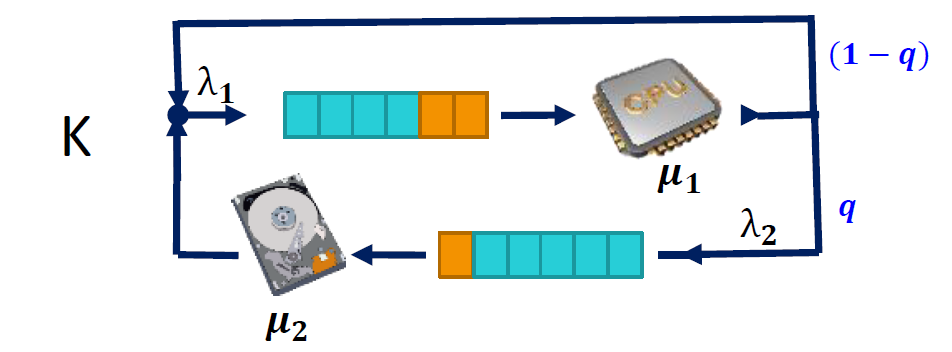
\includegraphics[width=\linewidth, keepaspectratio]{traccia}
  \caption{}
  \label{}
\end{figure}

\clearpage

\section{Soluzione}
Il sistema è composto da due sottosistemi($M=2$) e tre utenti($K=3$).\\
Il tasso di servizio del sistema uno ($\mu_1$) è 5 mentre quello del sistema due
($\mu_2$) è 2.\\
Il numero di possibili stati è pari al numero di modi di distribuire $K$ job in
$M$ sottosistemi.\\
$$ \binom{k+M-1}{M-1}=\binom{4}{1}=\frac{4!}{(4-1)!1!}=4$$
L'evoluzione della rete può essere descritta tramite un grafo della catena di Markov,
rappresentando i quattro stati con il numero di utenti presenti in ciascun sottosistema.\\

\begin{figure}[!htbp]
  \centering
  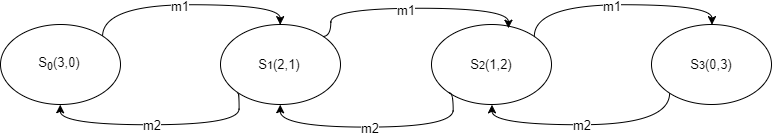
\includegraphics[width=\linewidth, keepaspectratio]{coda_elaborato_mkc}
  \caption{Grafo associato alla catena di Markov}
  \label{}
\end{figure}

Applicando l'equazione di conservazione del flusso su tutti i sottosistemi si
ottiene:
$$
\begin{cases}\lambda_2 = q\lambda_1 \\
\lambda_1 = (1-q)\lambda_1 + \lambda_2 \\
\end{cases}
$$


Risolvendo il sistema si ottiene:

$$ \lambda_1 = \lambda_1 $$

L'unica informazione che è possibile ricavare è:
$$ \lambda_2 = q \lambda_1 \ \ \Longrightarrow \ \ q=\frac{\lambda_2}{\lambda_1}$$
Essendo $q = \frac{1}{3} $ una possibile soluzione è:
$$
\begin{cases}
\widehat{\lambda}_2 = 1 \\
\widehat{\lambda}_1 = 3
\end{cases}
$$

\clearpage

\subsection{Gordon-Newell}
La soluzione proposta da \textbf{Gordon} e \textbf{Newell} permette di calcolare
la probabilità di trovarsi in ciascuno degli stati descritti dalla catena di Markov.\\
Dunque:
$$ p(n)=
\begin{cases}
  \frac{1}{G(K,M)}\prod_{i=0}^M \widehat{p}_i^{n_i} \ \ \ when \ \sum_{i}n_i = K\\
  0 \ \ \ \ \ \ \ \ \ \ \ \ \ \ \ \ \ \ \ \ \ \ \ when \ \sum_{i}n_i \neq K
\end{cases}
$$
Dove $G(K,M)$ è la condizione di normalizzazione.
$$ G(K,M)=\sum_{n : \sum_{i}n_i=K} \prod_{i=1}^M \widehat{p}_i^{n_i}$$


\subsubsection{Calcolo manuale}

I fattori di utilizzo dei singoli sottosistemi sono:

$$\widehat{\rho}_1 = \frac{\widehat{\lambda}_1}{\mu_1}=\frac{3}{5} $$
$$\widehat{\rho}_2 = \frac{\widehat{\lambda}_2}{\mu_2}=\frac{1}{2}$$

Applicando il teorema di \textbf{Gordon-Newwll}:
$$
\begin{cases}
  p_{3,0} = \frac{1}{G} \widehat{\rho}_1^3 \\
  p_{2,1} = \frac{1}{G} \widehat{\rho}_1^2 \widehat{\rho}_2 \\
  p_{1,2} = \frac{1}{G} \widehat{\rho}_1 \widehat{\rho}_2^2 \\
  p_{0,3} = \frac{1}{G} \widehat{\rho}_2^3 \\
\end{cases}
$$

Il valore di $G$ è:

$$ G = \widehat{\rho}_1^3  +  \widehat{\rho}_1^2 \widehat{\rho}_2 + \widehat{\rho}_1 \widehat{\rho}_2^2 + \widehat{\rho}_2^3 = 0,6710$$

La probabilità di essere in ogni stato è:

$$
\begin{cases}
  p_{3,0} = \frac{1}{0,6710} * (\frac{3}{5})^3=32,19\%\\
  p_{2,1} =  \frac{1}{0,6710} * (\frac{3}{5})^2*\frac{1}{2}=26,83\%\\
  p_{1,2} = \frac{1}{0,6710} * \frac{3}{5}*(\frac{1}{2})^2=22,25\%\\
  p_{0,3} = 1,4903 *\frac{1}{0,6710} * (\frac{1}{2})^3=18,13\%\\
\end{cases}
$$

Per calcolare il numero di job medio presenti in ogni sottosistema, conoscendo
la probabilità di essere in ciascuno stato, si utilizza la seguente relazione:

$$ E[N_i] = \sum_{i=0}^n p_i\cdot N_i $$

Quindi:

$$ E[N_1] = 3 \cdot p_{3,0} + 2 \cdot p_{2,1} + 1 \cdot p_{1,2} + 0 \cdot p_{0,3}=1,7258$$
$$ E[N_1] = 0 \cdot p_{3,0} + 1 \cdot p_{2,1} + 2 \cdot p_{1,2} + 3 \cdot p_{0,3}=1,2742$$
\vspace{1cm}
\subsubsection{Matlab}
Di seguito è riportata la funzione implementata in \textit{Matlab} della
soluzione proposta da \textbf{Gordon} e \textbf{Newell}.\\
\lstinputlisting[language=Matlab, caption={Funzione Gordon-Newell Matlab}, label={fun1}]{GordonNewell.m}

Per l'esecuzione della funzione mostrata nel listato \ref{fun1}, è stato implementato
il seguente script Matlab, il quale esegue la funzione \textit{GordonNewell}
per il calcolo delle probabilità di essere in ciascuno dei quattro stati del sistema
e successivamente calcola \textit{Numero medio di job} dei due sottosistemi.\\

\clearpage

\lstinputlisting[language=Matlab, caption={Script per il calcolo di Tempo medio di riposta, Numero medio di job e $\lambda$}, label={script1}]{CalcoloParametriSistemaGordonNewell.m}

\vspace{0.4cm}
L'output dello script \ref{script1} è il seguente:

\color{black} \begin{verbatim}
K =
3

M =
2

l1 =
3

l2 =
1

m1 =
5

m2 =
2

numerostati =
4

p30 =
0.3219

p21 =
0.2683

p12 =
0.2235

p03 =
0.1863

N1 =
1.7258

N2 =
1.2742
\end{verbatim} \color{black}

\subsection{Mean Value Analysis}
L'algoritmo di \textbf{Mean Value Analysis} permette di ottenere \textbf{\textit{numero di utenti}},
\textbf{\textit{tasso di servizio}} e \textbf{\textit{$\lambda_i$}}.

\vspace{0.3cm}

Caso base:\\
 \begin{center}
   $\overline{N}_i[0]=0  $ il sistema è vuoto.
 \end{center}

\vspace{0.2cm}

Ricorsione:
$$ \overline{T}_i[K]=(1+\overline{N}_i[K-1])\cdot \frac{1}{\mu_i}$$
$$ \overline{N}_i[K]=K\cdot \frac{\widehat{\lambda}_i\cdot \overline{T}_i[K]}{\sum_{j=1}^M \widehat{\lambda}_j \cdot \overline{T}_j[K]}$$
$$ \lambda_i[k]=\frac{\overline{N}_i[k]}{\overline{T}_i[k]}$$
\clearpage
\subsubsection{Calcolo manuale}
Considerando l'algoritmo ricorsivo si riportano i calcoli effettuati per il calcolo
di $\overline{N}_1$,  $\overline{N}_2$, $\overline{T}_1$,  $\overline{T}_2$,  $\lambda_1$ e $\lambda_2$.\\

\begin{tabular}{c|c|c}
\textbf{Numero job}&\textbf{Sottosistema 1}&\textbf{Sottosistema 2}\\
\hline
\hline
\rule[-4mm]{0mm}{1cm}
\multirow{3}*{K=1} &$ \overline{T}_1[1]=(1+0)\cdot \frac{1}{5}=0,2$ & $ \overline{T}_2[1]=(1+0)\cdot \frac{1}{2}=0,5$\\
\cline{2-3}
\rule[-4mm]{0mm}{1cm}
&$ \overline{N}_1[1]=1\cdot \frac{3\cdot 0,2}{3 \cdot 0,2 + 1 \cdot 0,5}=0,5455$ & $ \overline{N}_2[1]=1\cdot \frac{1 \cdot 0,5}{3 \cdot 0,2 + 1 \cdot 0,5}=0,4545$\\
\cline{2-3}
\rule[-4mm]{0mm}{1cm}
&$ \lambda_1[1]=\frac{0,5455}{0,2}=2,7275$ & $ \lambda_2[1]=\frac{0,4545}{0,2}=2,2725$\\
\hline
\hline
\rule[-4mm]{0mm}{1cm}
\multirow{3}*{K=2} &$ \overline{T}_1[2]=(1+0,5455)\cdot \frac{1}{5}=0,3091$ & $ \overline{T}_2[1]=(1+0,4545)\cdot \frac{1}{2}=0,7273$\\
\cline{2-3}
\rule[-4mm]{0mm}{1cm}
&$ \overline{N}_1[2]=2\cdot \frac{3\cdot 0,3091}{3 \cdot 0,3091 + 1 \cdot 0,7273}$= 1,1209 & $ \overline{N}_2[2]=2\cdot \frac{1\cdot 0,7273}{3 \cdot 0,3091 + 1 \cdot 0,7273}=0,8791$\\
\cline{2-3}
\rule[-4mm]{0mm}{1cm}
&$ \lambda_1[1]=\frac{1,1209}{0,3091}=3,6263$ & $ \lambda_2[1]=\frac{0,8792}{0,7273}=1,2089$\\
\hline
\hline
\rule[-4mm]{0mm}{1cm}
\multirow{3}*{K=3} &$ \overline{T}_1[3]=(1+1,1209)\cdot \frac{1}{5}=0,4242$ & $ \overline{T}_2[3]=(1+8791)\cdot \frac{1}{2}=0,9396$\\
\cline{2-3}
\rule[-4mm]{0mm}{1cm}
&$ \overline{N}_1[1]=3\cdot \frac{3\cdot 0,4242}{3 \cdot 0,4242 + 1 \cdot 0,9396}=1,7258$ & $ \overline{N}_2[3]=3\cdot \frac{1\cdot 0,9396}{3 \cdot 0,4242 + 1 \cdot 0,9396}=1,2742$\\
\cline{2-3}
\rule[-4mm]{0mm}{1cm}
&$ \lambda_1[1]=\frac{1,7258}{0,4242}=4,0684$ & $ \lambda_2[1]=\frac{1,2742}{0,9296}=1,3561$\\
\hline
\end{tabular}

\clearpage

\subsubsection{Matlab}
Di seguito è riportata la funzione implementata in \textit{Matlab} dell'algoritmo
della \textbf{Mean Value Analisys}.\\
\lstinputlisting[language=Matlab, caption={Funzione Mean Value Analsys Matlab}, label={fun}]{mva.m}

Per l'esecuzione della funzione mostrata nel listato \ref{fun}, è stato implementato
 il seguente script Matlab, il quale esegue la funzione \textit{mva} con $K=3$ e
 ne mostra l'output ed infine esegue la \textbf{\textit{Mean Value Analysis}} con
 $K=50$ e mostra i grafici relativi a \textit{Tempo medio di Risposta}, \textit{Numero medio di job} e $\lambda$
 dei due sottosistemi.\\

\lstinputlisting[language=Matlab, caption={Script per il calcolo di Tempo medio di riposta, Numero medio di job e $\lambda$}, label={script2}]{CalcoloParametriSistemaMVA.m}

\vspace{0.4cm}
L'output dello script \ref{script2} è il seguente:

\color{black} \begin{verbatim}
K =
3

M =
2

l =
3     1

m =
5     2

T =
0.2000    0.5000
0.3091    0.7273
0.4242    0.9396

N =
0.5455    0.4545
1.1209    0.8791
1.7258    1.2742

L =
2.7273    0.9091
3.6264    1.2088
4.0686    1.3562
\end{verbatim} \color{black}

\begin{figure}[!htbp]
  \centering
  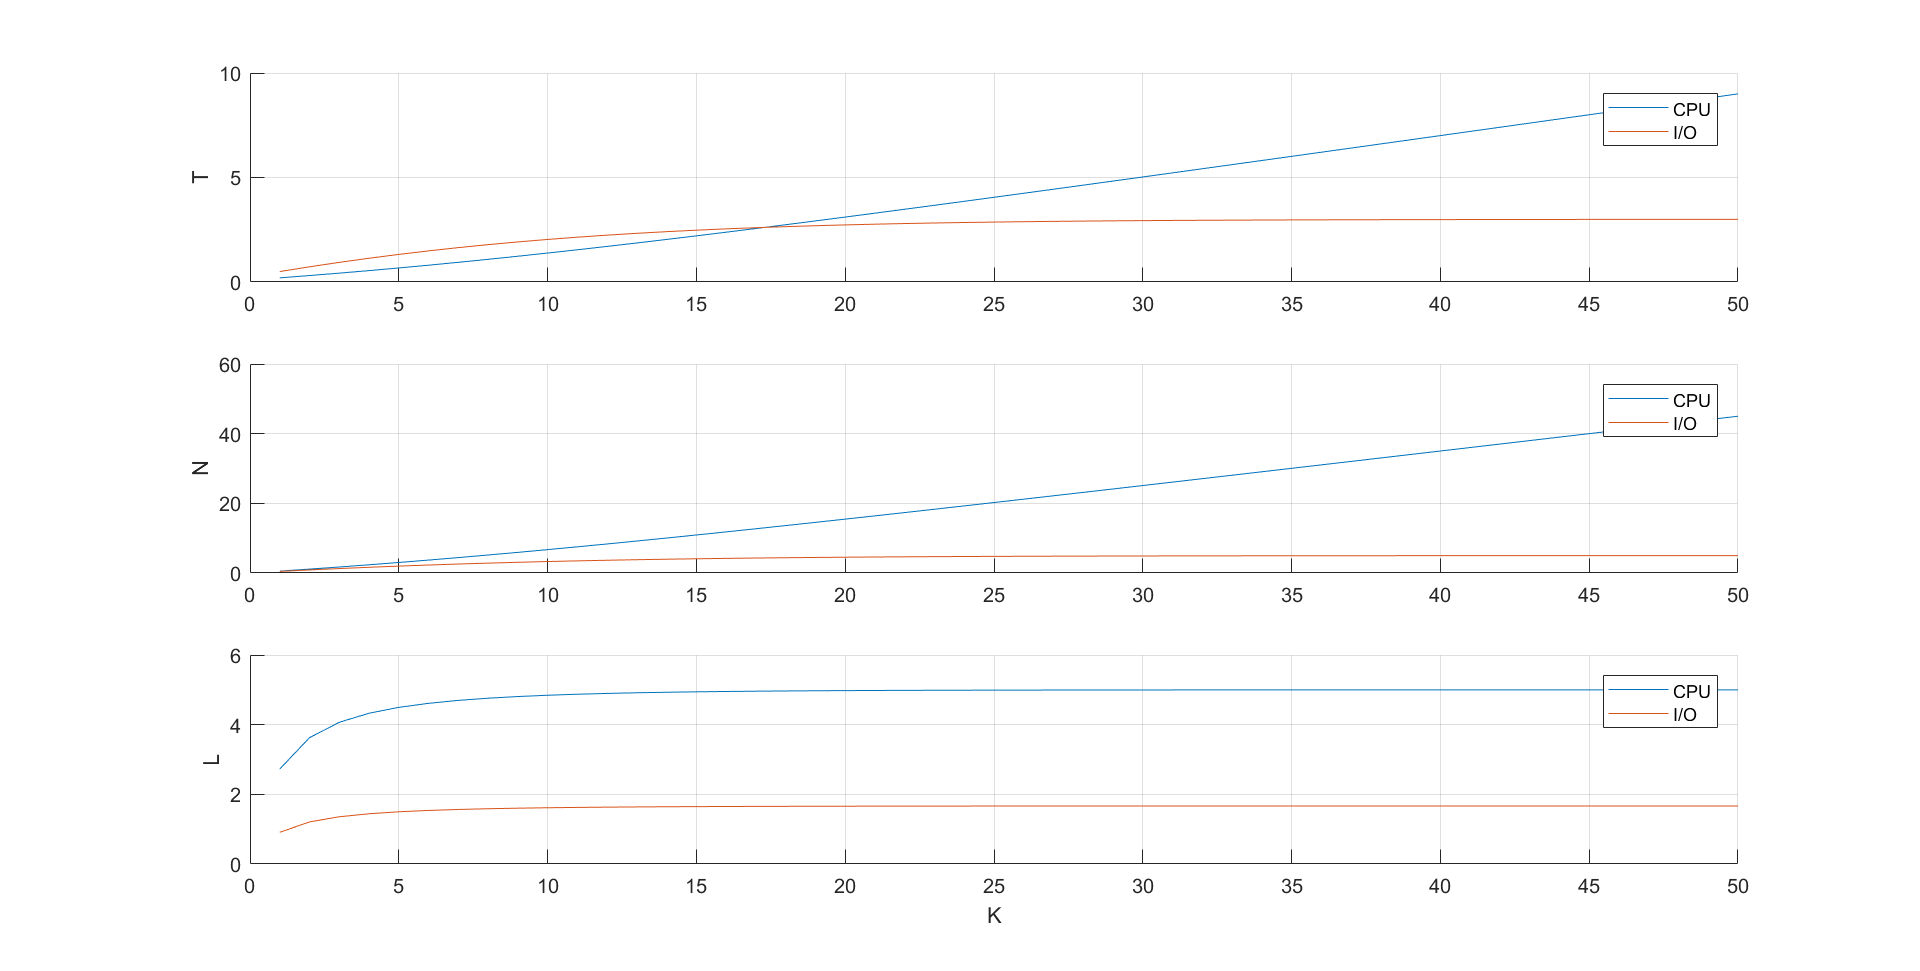
\includegraphics[width=\linewidth, keepaspectratio]{grafico}
  \caption{Grafico Tempo medio di riposta, Numero medio di job e $\lambda$}
  \label{graph1}
\end{figure}

Dal grafico in \figurename~\ref{graph1} si osserva che da $K=17$ il tempo di risposta medio
della CPU diviene maggiore di quello dell'I/O, ciò può essere attribuito al
raggiungimento del tesso di risposta massimo della CPU la quale essendo in serie
con l'I/O  funge da collo di bottiglia, quindi se si volessero migliorare le prestazione
del sistema bisognerebbe utilizzare una CPU con un tasso di risposta maggiore.\\
Di fatti il sottosistema uno ha fattore di utilizzo maggiore del sottosistema due
quindi incrementando di un'unità il tasso di servizio della CPU le prestazioni
risultano migliori in quanto i due sistemi avranno lo stesso tasso di utilizzo.\\

\begin{figure}[!htbp]
  \centering
  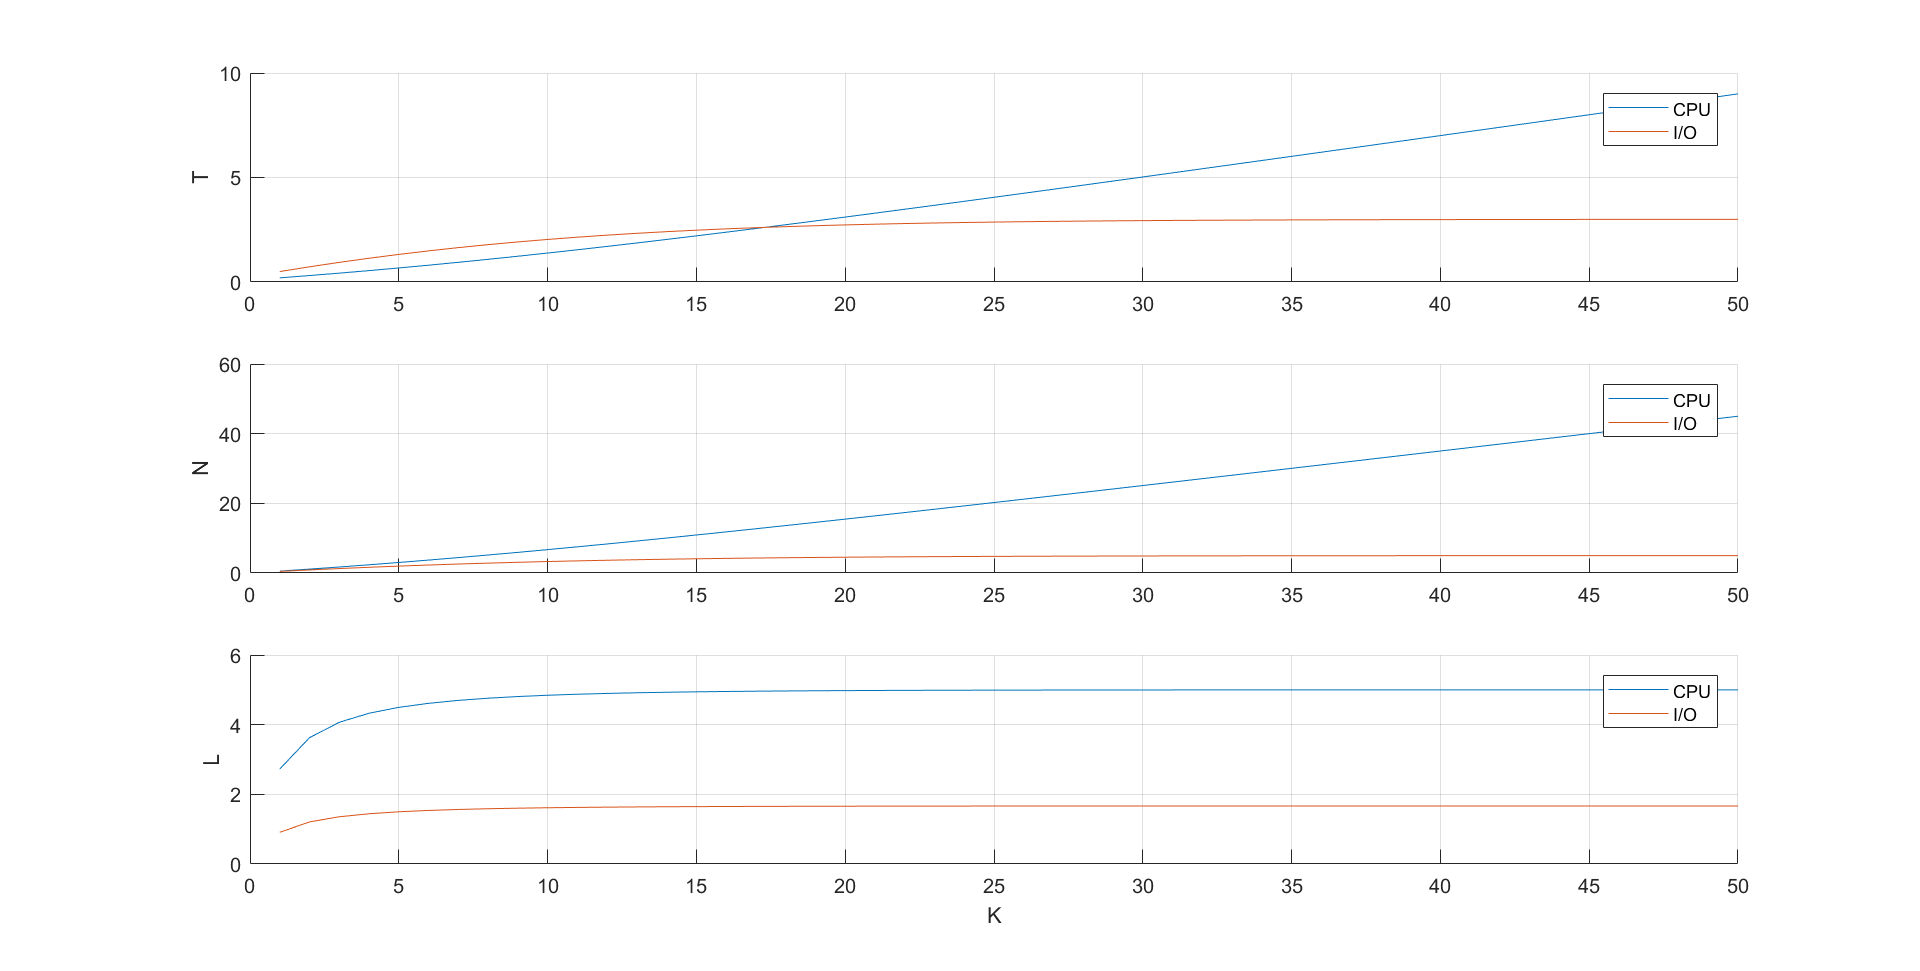
\includegraphics[width=\linewidth, keepaspectratio]{grafico}
  \caption{Grafico Tempo medio di riposta, Numero medio di job e $\lambda$, con $\mu_1=6$}
  \label{graph1}
\end{figure}
